\section{Architettura}
Lo scopo di questa sezione è di descrivere l'architettura e i design pattern\glosp utilizzati.
\subsection{Design pattern}
\begin{figure}[H]
	\centering
	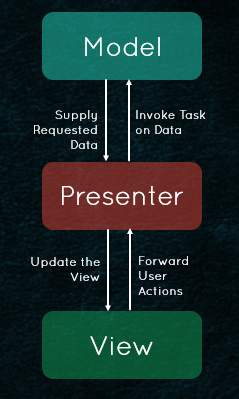
\includegraphics[width=0.3\textwidth]
	{res/images/mvp.png}\\
	\caption{Schema MVP}
	\label{Schema MVP}
\end{figure}
P2PCS implementa il design pattern MVP\glosp seguendo le linee guida fornite da Google\glosp e reperibili al seguente link: \url{https://github.com/googlesamples/android-architecture}.
\newline
\subsubsection{Model}
Contiene i dati che l’applicazione può elaborare e visualizzare. Mette inoltre a disposizione metodi per leggere e modificare tali dati.
In questo progetto vengono forniti i metodi di lettura e scrittura su Firebase\glo.
Il model è dotato di tre servizi principali, successivamente segmentati in macro-argomenti, che sono:
\begin{itemize}
	\item Authentication;
	\item Database;
	\item Storage.
\end{itemize}

Per manutenere il model è necessario accedere al package \textbf{model} e agire sui rispettivi file \textbf{BrandModel} e \textbf{FirebaseModel}.
\subsubsection{View}
Rappresenta l’interfaccia utente. Ogni View\glosp disegna sul dispositivo una schermata che permette all'utente di interagire con l’applicazione.

La View è composta da varie Activity\glosp e Fragment\glosp il cui layout è definito nel package \textbf{layout} mentre l'implementazione è suddivisa nei vari package precedentemente descritti.
\subsubsection{Presenter}
È il mediatore tra Model\glosp e View\glosp ed elabora i dati del Model in modo che possano essere visualizzati nella View e risponde alle richieste dell'utente nella View interagendo con il Model. Il Presenter\glosp quindi vuole tenere separate la parte grafica dell'applicazione e la logica di business.\newline
Ogni activity\glosp quindi sarà composta da una View e un Presenter che saranno legati da un contratto che ne definisce le rispettive interfacce.
\begin{figure}[H]
	\centering
	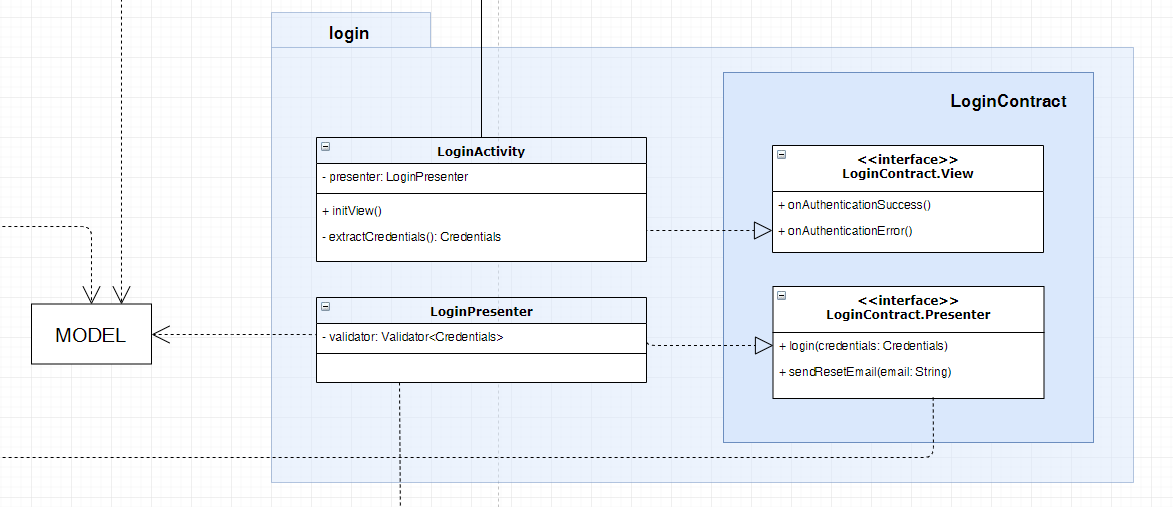
\includegraphics[width=0.9\textwidth]
	{res/images/contratto.png}\\
	\caption{Diagramma d'esempio del login}
	\label{Schema Login}
\end{figure}
\newpage
\subsection{Directory tree}
\begin{figure}[H]
	\centering
	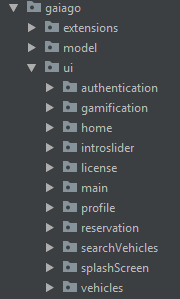
\includegraphics[width=0.3\textwidth]
	{res/images/directorytree.png}\\
	\caption{Directory tree}
	\label{Directory Tree}
\end{figure}
\begin{itemize}
	\item \textbf{extension}: contiene classi e funzioni di utilità come la conversione di una data in millisecondi ad una data in formato ddMMyyyy;
	\item \textbf{model}: contiene i package\glo, classi e interfacce che si occupano della gestione di Firebase\glo;
	\item \textbf{ui}: contiene la user interface suddividendola in macro-package.
\end{itemize}
\begin{figure}[H]
	\centering
	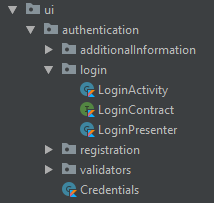
\includegraphics[width=0.3\textwidth]
	{res/images/authentication.png}\\
	\caption{Authentication package}
	\label{Authentication package}
\end{figure}
Ogni macro-package è infine suddiviso in package\glosp che rappresentano le singole funzionalità dell'applicazione, questi sono composti principalmente da View\glo, Presenter\glosp e Contract\glo. Alcuni package possono contenere fragment\glosp aggiuntivi.

\newpage

\subsection{Elenco Activity}
Al fine di una manutenzione efficace di View e Presenter verranno descritti i singoli package.

\subsubsection{Authentication}
Contiene tutti i package che interessano l'accesso di un utente non autenticato all'applicazione.
\begin{itemize}
	\item \textbf{additional information}: aggiunta di informazioni personali a seguito della registrazione;
	\item \textbf{login}: autenticazione di un utente già registrato;
	\item \textbf{registration}: registrazione di un utente non autenticato;
	\item \textbf{validators}: in questo package sono contenuti tutti i validatori dei campi dati come email e password.	
\end{itemize}
\subsubsection{Gamification}
\begin{itemize}
	\item \textbf{dailyRewards}: assegnazione premi giornalieri;
	\item \textbf{leaderBoard}: classifica utenti per punteggio;
	\item \textbf{milestoneUnlock}: assegnazione di premi in base al punteggio dell'utente;
	\item \textbf{minigame}: minigioco con veicolo personalizzabile dall'utente.
\end{itemize}
\subsubsection{Home}
Prima Activity visualizzata da un utente autenticato, si compone di uno slider con due fragment\glo.
\subsubsection{Introslider}
Guida introduttiva che avviene a seguito della registrazione.
\subsubsection{License}
Package che gestisce l'aggiunta della patente di guida da parte dell'utente.
Contiene:
\begin{itemize}
	\item \textbf{dates}: per l'inserimento delle date di rilascio e scadenza;
	\item \textbf{number}: per l'inserimento del numero della patente;
	\item \textbf{pictures}: per l'inserimento delle foto della patente.
\end{itemize}
\subsubsection{Main}
Contiene l'Activity\glosp principale dell'applicazione e su cui si appoggia l'intera struttura. In essa vengono istanziate i cinque fragment\glosp principali che rappresentano: home, lista veicoli, ricerca veicoli, area personale e Gamification\glo.
\subsubsection{Profile}
Contiene tutti i package e le activity che si occupano della gestione dell'area personale.
\subsubsection{Reservations}
Contiene tutti i package e le activity per la gestione delle prenotazioni.
Contiene:
\begin{itemize}
	\item \textbf{reservationsList}: si occupa della visualizzazione della lista delle prenotazioni;
	\item \textbf{showReservation}: consente la visualizzazione nel dettaglio di una singola prenotazione.
\end{itemize}
\subsubsection{SearchVehicles}
Per la ricerca di un veicolo, contiene \textbf{searchResultsSlider} che si articola in:
\begin{itemize}
	\item \textbf{availableVehiclesList}: per la visualizzazione di una lista dei veicoli disponibili;
	\item \textbf{vehiclesMap}: i veicoli vengono mostrati tramite marker su una mappa.
\end{itemize}
\subsubsection{SplashScreen}
Prima activity in assoluto visualizzata da un utente generico si occupa di identificare l'utente e rimandarlo opportunamente al login o all'activity principale.
\subsubsection{Vehicles}
Package per la gestione dei veicoli. Si compone di:
\begin{itemize}
	\item \textbf{addVehicle}: per l'aggiunta di un veicolo;
	\item \textbf{showVehicle}: per la visualizzazione di un singolo veicolo;
	\item \textbf{vehicleList}: per la visualizzazione di una lista dei propri veicoli.
\end{itemize}